\documentclass[conference]{IEEEtran}
\IEEEoverridecommandlockouts
\usepackage{cite}
\usepackage{amsmath,amssymb,amsfonts}
\usepackage{algorithmic}
\usepackage{graphicx}
\usepackage{textcomp}
\usepackage{xcolor}
\def\BibTeX{{\rm B\kern-.05em{\sc i\kern-.025em b}\kern-.08em
    T\kern-.1667em\lower.7ex\hbox{E}\kern-.125emX}}
\begin{document}

\title{Movie Recommendation System Using Collaborative Filtering: A Comparative Study of User-Based, Item-Based, and Matrix Factorization Approaches}

\author{\IEEEauthorblockN{Taibaz Pathan}
\IEEEauthorblockA{\textit{Department of Computer Science} \\
\textit{Frankfurt University of Applied Sciences}\\
Frankfurt am Main, Germany \\
Student ID: 284085 \\
taibaz.pathan@stud.fra-uas.de \\
Supervisor: Prof. Dr. Andreas Pech}
}

\maketitle

\begin{abstract}
This report presents the design, implementation, and evaluation of a movie recommendation system built on the MovieLens ml-latest-small dataset (100,836 ratings, 610 users, 9,742 movies). Two collaborative filtering approaches were implemented from first principles: User-Based Collaborative Filtering (UBCF) using Pearson correlation, and Item-Based Collaborative Filtering (IBCF) using adjusted cosine similarity. Both were compared against three non-personalized baselines (global, user, and item mean predictors) and a matrix factorization approach (SVD). After hyperparameter tuning via grid search, UBCF achieved the lowest prediction error (RMSE = 0.8430) while SVD achieved the best overall performance across both accuracy and ranking metrics (RMSE = 0.8379, Precision@10 = 0.0601). A paired bootstrap significance test ($n=1000$ resamples) confirmed that UBCF's advantage over IBCF is statistically significant (95\% CI [0.0252, 0.0418], excluding zero). All personalized models outperformed the three non-personalized baselines by a clear margin, which is the result collaborative filtering is expected to produce if it is working correctly. The study further investigates cold-start behavior, sparsity sensitivity, and computational scalability, and documents two implementation defects discovered and corrected during development: an incorrect rating-aggregation formula in IBCF and a prediction-saturation artifact in UBCF. The implementation includes 104 automated tests and is version-controlled for reproducibility.
\end{abstract}

\begin{IEEEkeywords}
collaborative filtering, recommender systems, MovieLens, user-based CF, item-based CF, matrix factorization, SVD, RMSE, precision-recall
\end{IEEEkeywords}

\section{Introduction}

\subsection{Motivation}
Streaming catalogs now contain far more titles than a user can realistically browse, and many users abandon a session without picking anything simply because there are too many options. Recommender systems address this by using a user's past ratings, together with the ratings of similar users, to narrow a large catalog down to a short, relevant list. Collaborative filtering (CF) is one of the most common approaches to this problem and is used in production by companies such as Netflix and Amazon. Its main advantage over content-based methods is that it needs no manual tagging of items --- relevance is inferred entirely from patterns in the user-item rating matrix.

\subsection{Problem Statement}
Given a sparse matrix of historical user ratings for movies, the task is to predict the rating a user would give to a movie they have not yet seen, and to use these predictions to build a ranked list of recommendations. Three things make this non-trivial: extreme data sparsity (98.3\% of the user-item matrix is unobserved in the raw dataset), the cold-start problem for users and items with few ratings, and the fact that a low prediction error does not automatically mean a good ranked list --- accuracy and ranking quality have to be evaluated separately.

\subsection{Objectives}
\begin{itemize}
\item Implement User-Based and Item-Based Collaborative Filtering from first principles, without relying on pre-built similarity or prediction functions.
\item Evaluate both approaches using both rating-accuracy metrics (RMSE, MAE) and ranking-quality metrics (Precision@K, Recall@K, F1@K).
\item Establish non-personalized baselines to quantify the actual value added by personalization.
\item Tune model hyperparameters systematically via grid search rather than manual selection.
\item Extend the comparison to a matrix factorization approach (SVD) as a third algorithmic family.
\item Analyze system behavior under cold-start and sparse-data conditions, and characterize computational scalability.
\item Produce a reproducible, tested, version-controlled implementation.
\end{itemize}

\subsection{Report Structure}
Section II reviews related work on collaborative filtering. Section III covers the dataset, preprocessing, the algorithms themselves, and how they were evaluated. Section IV presents the results: model comparison, a significance test, hyperparameter tuning, cold-start behavior, and scalability. Section V discusses two implementation issues found during development and the limitations of the current system, and Section VI concludes with directions for future work.

\section{Background and Related Work}
Collaborative filtering methods are broadly divided into memory-based and model-based approaches. Memory-based methods, which include both UBCF and IBCF, compute predictions directly from the raw rating matrix using similarity measures, without learning a compressed intermediate representation. Resnick et al.~\cite{b1} introduced the neighborhood-based formulation for user-based CF used in this project, in which a target user's rating is predicted as a similarity-weighted average of deviations from neighboring users' mean ratings. Sarwar et al.~\cite{b2} later showed that item-based approaches, which compute similarity between items rather than users, offer comparable or superior accuracy while being more computationally stable, since item-item relationships change more slowly over time than user-user relationships. Model-based approaches, by contrast, learn latent factor representations of users and items; singular value decomposition (SVD), popularized during the Netflix Prize competition~\cite{b5}, is one of the most widely used techniques in this family and is included in this study as a point of comparison.

\section{Methodology}

\subsection{Dataset}
The MovieLens ml-latest-small dataset~\cite{b3} was used throughout this project. It contains 100,836 ratings on a 0.5--5.0 scale (in 0.5 increments), submitted by 610 users for 9,742 movies between March 1996 and September 2018. Exploratory analysis of the raw dataset revealed three properties with direct implications for model design. First, the mean rating (3.50) sits well above the scale midpoint (2.75), indicating a positive rating bias consistent with users self-selecting content they expect to enjoy; this motivated the use of mean-centered similarity measures rather than raw rating comparison. Second, both user activity and movie popularity are heavily right-skewed: the median user has rated only 68 movies while the most active user has rated over 2,000, and the median movie has only 3 ratings. Third, the raw user-item matrix is 98.3\% sparse, meaning fewer than 2\% of all possible (user, movie) pairs have an observed rating.

\subsection{Data Preprocessing}
\label{sec:preprocessing}
To ensure that similarity computations were based on statistically meaningful sample sizes, an iterative filtering procedure was applied: users and movies with fewer than 20 ratings were removed, with the process repeated until convergence (since removing sparse movies can push previously-eligible users below the threshold, and vice versa). This reduced the dataset to 67,020 ratings across 566 users and 1,286 movies, with sparsity falling to 92.6\%. The filtered data was then split per-user into training and test sets using an 80/20 ratio, yielding 53,614 training ratings and 13,406 test ratings. Splitting per-user, rather than globally at random, guarantees that every user in the test set has a corresponding profile in the training set, which is a prerequisite for meaningful CF evaluation. A fixed random seed (42) was used throughout for reproducibility.

\subsection{Similarity Metrics}
Two similarity measures were implemented from scratch in NumPy, without using library functions such as \texttt{pandas.corr()} or scikit-learn's pairwise-similarity utilities. Cosine similarity treats each user's (or item's) rating vector as a geometric vector and measures the cosine of the angle between two vectors, with missing ratings excluded from the computation rather than treated as zero. Pearson correlation additionally mean-centers each vector before comparison, which corrects for users who rate systematically higher or lower than average. Following Resnick et al.~\cite{b1}, mean-centering was computed over the co-rated items only, not each user's full rating history, and a minimum co-rating threshold (\texttt{min\_support}) was enforced: similarity between two users (or items) with fewer co-ratings than this threshold was set to zero, since correlation computed from very few shared observations is statistically unreliable. Both metrics were implemented at the vector level (for single-pair computation) and at the matrix level (fully vectorized, for computing the complete similarity matrix in a single operation).

\subsection{User-Based Collaborative Filtering (UBCF)}
UBCF predicts a target user $u$'s rating for item $i$ as a similarity-weighted average of the deviations of $u$'s $K$ nearest neighbors from their own mean ratings, added back to $u$'s own mean rating:
\begin{equation}
\hat{r}_{ui} = \bar{r}_u + \frac{\sum_{v} sim(u,v)\cdot(r_{vi} - \bar{r}_v)}{\sum_{v} |sim(u,v)|}
\label{eq:ubcf}
\end{equation}
where the sum runs over the $K$ users most similar to $u$ who have also rated item $i$. Only users who have actually rated the target item are considered as candidate neighbors. Because \eqref{eq:ubcf} is a weighted average of unbounded deviations rather than a convex combination of ratings, its output is not mathematically guaranteed to remain within the original [0.5, 5.0] rating scale (see Section~\ref{sec:impl}); predictions are therefore clipped to this range post-hoc.

\subsection{Item-Based Collaborative Filtering (IBCF)}
IBCF predicts a rating by finding the $K$ items most similar to the target item that the target user has already rated, and combining the user's ratings for those items, weighted by item-item similarity. Following Sarwar et al.~\cite{b2}, item-item similarity was computed using adjusted cosine similarity: each rating is first centered by subtracting the rating user's mean (not the item's mean), which corrects for user-level rating-scale differences before comparing items. The prediction itself likewise uses item-mean-centered deviations, for the reasons discussed in Section~\ref{sec:impl}:
\begin{equation}
\hat{r}_{ui} = \bar{r}_i + \frac{\sum_{j} sim(i,j)\cdot(r_{uj} - \bar{r}_j)}{\sum_{j} |sim(i,j)|}
\label{eq:ibcf}
\end{equation}

\subsection{Matrix Factorization (SVD)}
As a third, model-based point of comparison, a matrix factorization model was implemented using the SVD algorithm provided by the scikit-surprise library~\cite{b4}, configured with 50 latent factors and 20 training epochs (random seed 42). Unlike UBCF and IBCF, SVD learns a dense low-dimensional embedding for each user and item via stochastic gradient descent, such that the dot product of a user's and item's embeddings approximates their rating. This model was not subjected to the same hyperparameter tuning process as UBCF and IBCF (Section~\ref{sec:tuning}); default, commonly-used settings were retained, which is noted as a limitation in Section~\ref{sec:limitations}.

\subsection{Baseline Models}
Three non-personalized baseline predictors were implemented to establish a lower bound on acceptable performance: Global Mean, which always predicts the overall average rating across the training set; User Mean, which predicts each user's own average rating regardless of item; and Item Mean, which predicts each item's own average rating regardless of user. A properly functioning personalized CF model is expected to outperform all three; failure to do so would indicate a fundamental implementation defect rather than a genuine modeling limitation.

\subsection{Evaluation Metrics}
Two categories of metric were used. Accuracy metrics --- Root Mean Square Error (RMSE) and Mean Absolute Error (MAE) --- measure how close predicted ratings are to actual ratings on the held-out test set. Ranking metrics --- Precision@K, Recall@K, and their harmonic mean F1@K --- were additionally implemented because RMSE alone does not capture what a recommender system is actually used for: presenting a short, ranked list of items. An item was defined as ``relevant'' to a user if their true rating for it was 4.0 or higher, following common MovieLens convention. Precision@K measures the fraction of a user's top-K recommendations that are relevant; Recall@K measures the fraction of all relevant items that appear within the top K.

\subsection{Hyperparameter Tuning}
\label{sec:tuning}
Both UBCF and IBCF expose two key hyperparameters: $k$, the neighborhood size, and \texttt{min\_support}, the minimum co-rating threshold. A grid search was performed over $k \in \{5, 10, 20, 30, 40\}$ and \texttt{min\_support} $\in \{1, 3, 5, 10\}$ --- 20 configurations per model, 40 total --- with each configuration evaluated on RMSE and Precision@10. Because rating-accuracy and ranking-quality do not necessarily optimize together, both the RMSE-optimal and Precision@10-optimal configurations were recorded for each model; Precision@10 was adopted as the primary selection criterion for the final configuration used in all subsequent experiments, since ranking quality is arguably the more practically relevant objective for a recommender system. The RMSE-optimal alternative is reported alongside it in Section~\ref{sec:tuning-results} for completeness.

\section{Results}

\subsection{Model Comparison}
Table~\ref{tab:comparison} reports RMSE, MAE, Precision@10, and Recall@10 for all six models --- the three baselines, tuned UBCF, tuned IBCF, and SVD --- evaluated on the same held-out test set of 13,406 ratings.

\begin{table}[htbp]
\caption{Final Comparison of All Six Models on the Held-Out Test Set (13,406 Ratings). ``ms'' = min\_support.}
\begin{center}
\begin{tabular}{|l|c|c|c|c|}
\hline
\textbf{Model} & \textbf{RMSE} & \textbf{MAE} & \textbf{P@10} & \textbf{R@10} \\
\hline
SVD (n\_factors=50) & 0.8379 & 0.6435 & 0.0601 & 0.0495 \\
\hline
UBCF (k=20, ms=10) & 0.8430 & 0.6407 & 0.0499 & 0.0453 \\
\hline
IBCF (k=30, ms=1) & 0.8769 & 0.6731 & 0.0562 & 0.0382 \\
\hline
User Mean & 0.9128 & 0.7064 & 0.0250 & 0.0246 \\
\hline
Item Mean & 0.9253 & 0.7152 & 0.0365 & 0.0346 \\
\hline
Global Mean & 0.9990 & 0.8000 & 0.0250 & 0.0246 \\
\hline
\end{tabular}
\label{tab:comparison}
\end{center}
\end{table}

\begin{figure}[htbp]
\centerline{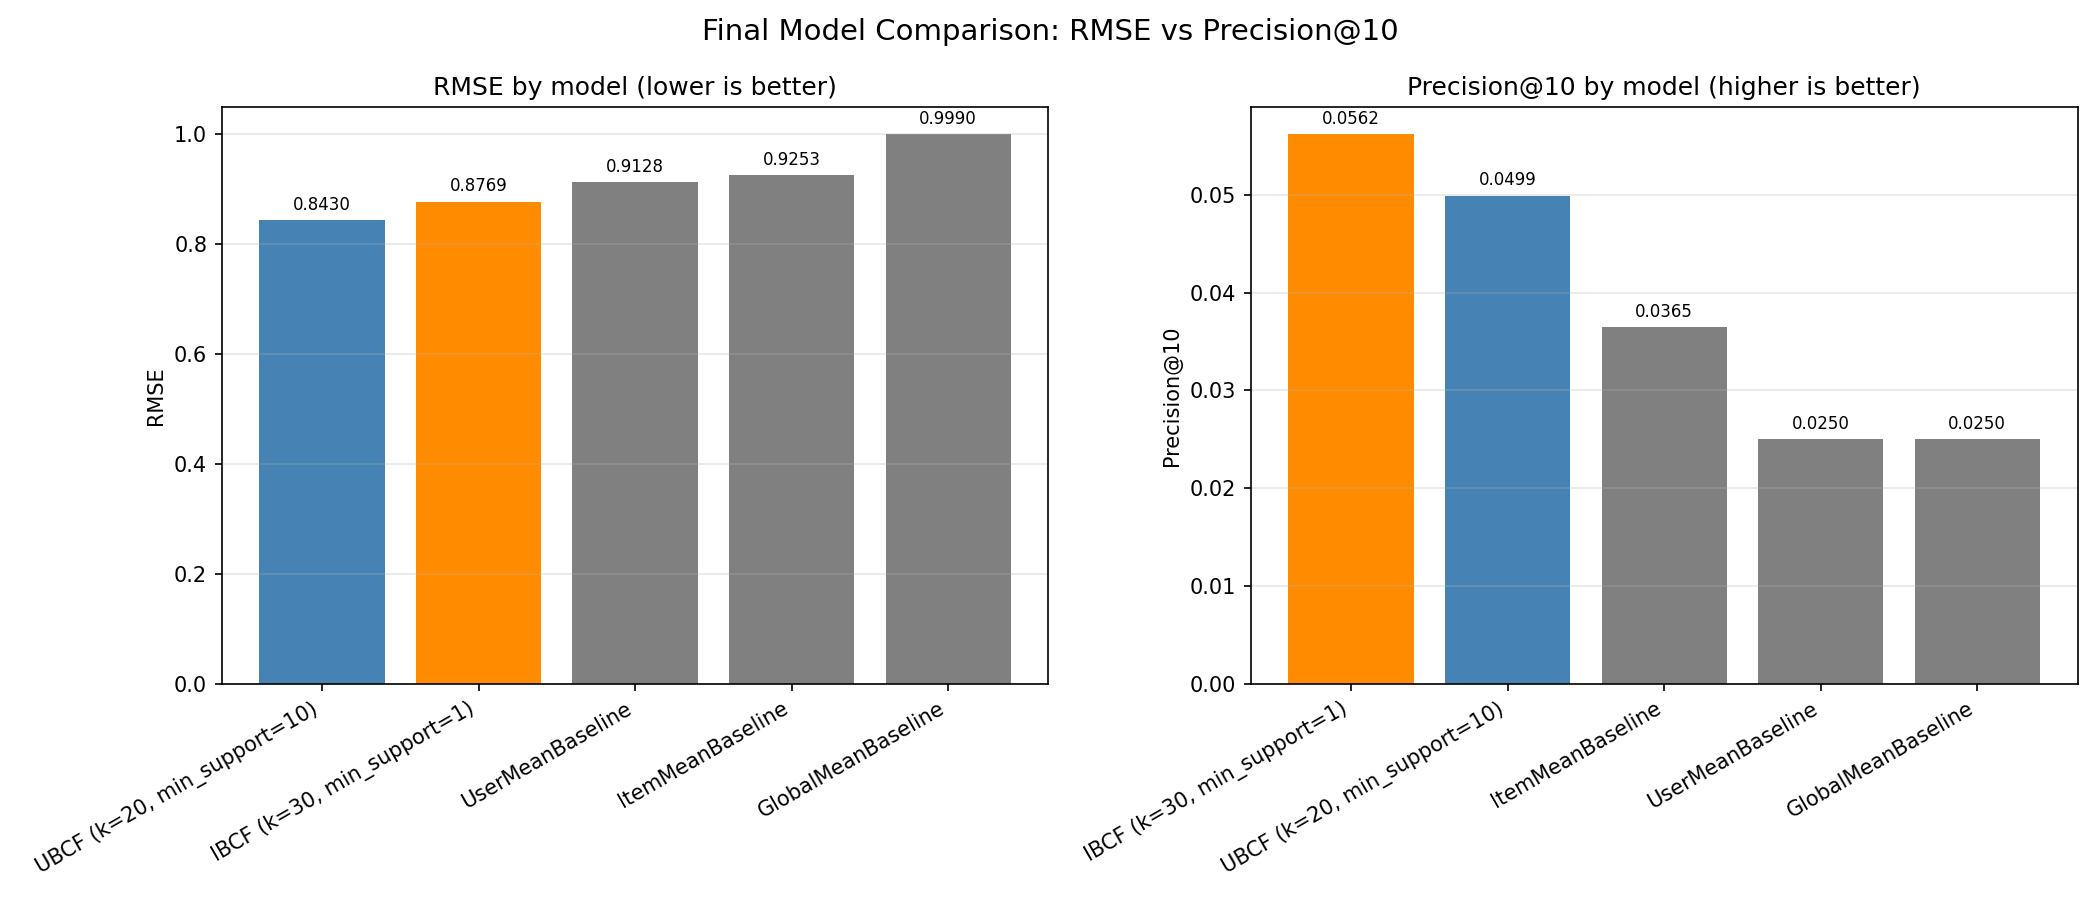
\includegraphics[width=\linewidth]{figures/final_model_comparison.png}}
\caption{RMSE and Precision@10 across all six models.}
\label{fig:comparison}
\end{figure}

Fig.~\ref{fig:comparison} plots the same RMSE and Precision@10 values. All three personalized models (SVD, UBCF, IBCF) outperform all three non-personalized baselines on every metric, which shows that the personalization signal in this dataset is real and not just noise. SVD achieves the best RMSE, MAE, Precision@10, and Recall@10 simultaneously; this is directionally consistent with Koren et al.~\cite{b5}, who report that matrix factorization tends to outperform neighborhood-based methods on the much larger Netflix Prize dataset, although this project does not independently establish that the same advantage holds at ml-latest-small's scale. Between the two neighborhood-based methods, UBCF achieves the lower RMSE while IBCF achieves the higher Precision@10, showing that rating-accuracy and ranking-quality are related but not the same objective, and can favor different models.

\subsection{Statistical Significance of the UBCF--IBCF Difference}
To determine whether UBCF's RMSE advantage over IBCF (0.8430 vs. 0.8769) reflects a genuine algorithmic difference or sampling variation from the particular train/test split, a paired bootstrap significance test was performed. Per-prediction squared errors for both models were resampled with replacement 1,000 times (identical resample indices applied to both models), and RMSE was recomputed on each resample. UBCF achieved lower RMSE than IBCF in 100\% of the 1,000 resamples. The 95\% confidence interval for the RMSE difference (IBCF $-$ UBCF) was [0.0252, 0.0418], which excludes zero. This supports the conclusion that UBCF's advantage over IBCF is statistically significant rather than a product of the particular train/test split.

\subsection{Hyperparameter Tuning Results}
\label{sec:tuning-results}
Table~\ref{tab:tuning} summarizes the outcome of the 40-configuration grid search described in Section~\ref{sec:tuning}, and Fig.~\ref{fig:tuning} plots RMSE and Precision@10 across the full range of $k$ for each \texttt{min\_support} value. For both models, the RMSE-optimal and Precision@10-optimal configurations differ, which shows that the two objectives do not have the same optimum.

\begin{table}[htbp]
\caption{RMSE-Optimal vs. Precision@10-Optimal Hyperparameter Configurations. The Precision@10-Optimal Configuration Was Adopted for All Subsequent Experiments.}
\begin{center}
\begin{tabular}{|l|c|c|c|c|}
\hline
\textbf{Model / Criterion} & \textbf{k} & \textbf{ms} & \textbf{RMSE} & \textbf{P@10} \\
\hline
UBCF --- best RMSE & 40 & 5 & 0.8371 & 0.0406 \\
\hline
UBCF --- best P@10 (used) & 20 & 10 & 0.8430 & 0.0499 \\
\hline
IBCF --- best RMSE & 20 & 3 & 0.8729 & 0.0522 \\
\hline
IBCF --- best P@10 (used) & 30 & 1 & 0.8769 & 0.0562 \\
\hline
\end{tabular}
\label{tab:tuning}
\end{center}
\end{table}

\begin{figure}[htbp]
\centering
\begin{minipage}{0.48\linewidth}
\centering
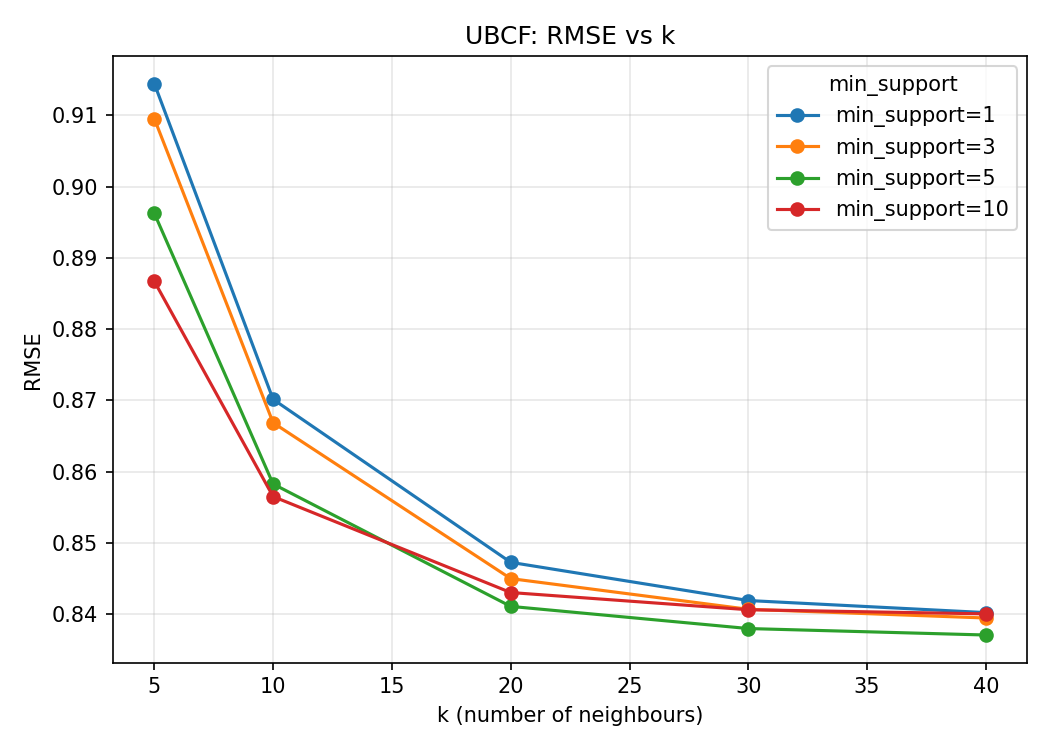
\includegraphics[width=\linewidth]{figures/ubcf_rmse_vs_k.png}
\end{minipage}
\hfill
\begin{minipage}{0.48\linewidth}
\centering
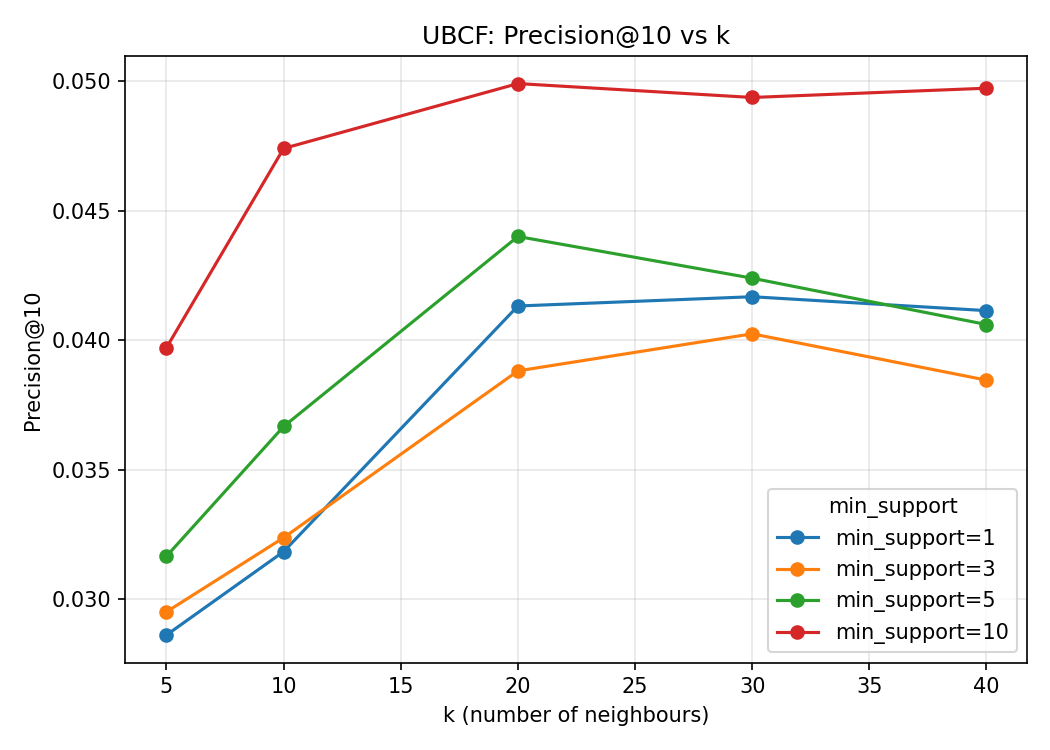
\includegraphics[width=\linewidth]{figures/ubcf_precision_vs_k.png}
\end{minipage}

\vspace{4pt}

\begin{minipage}{0.48\linewidth}
\centering
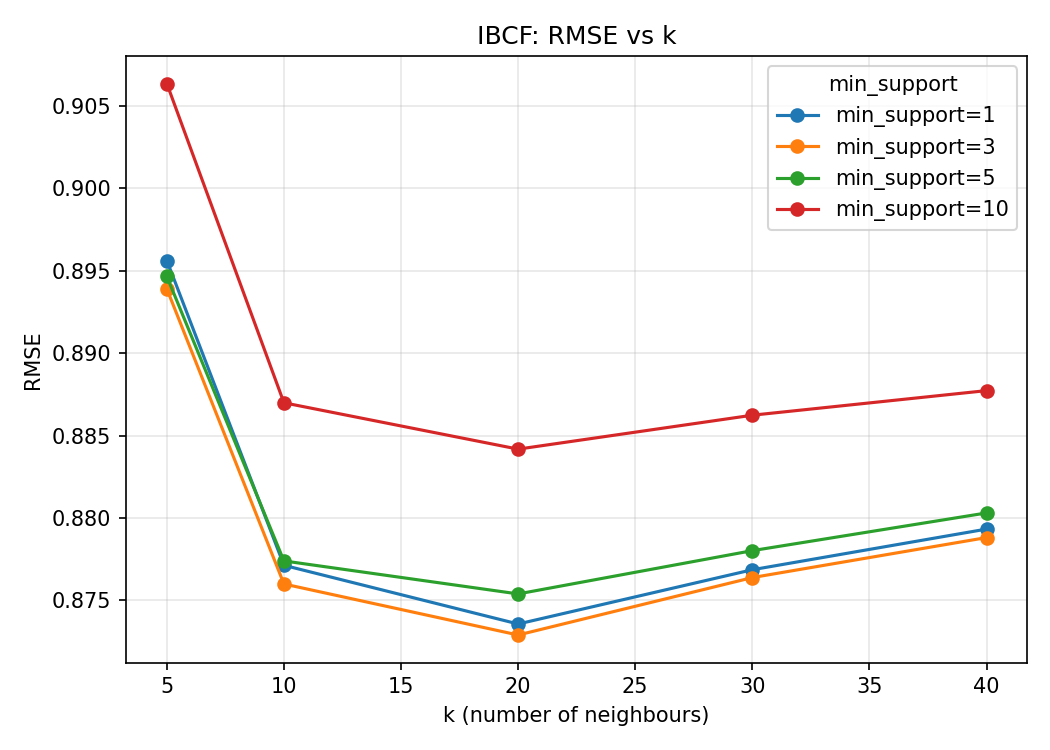
\includegraphics[width=\linewidth]{figures/ibcf_rmse_vs_k.png}
\end{minipage}
\hfill
\begin{minipage}{0.48\linewidth}
\centering
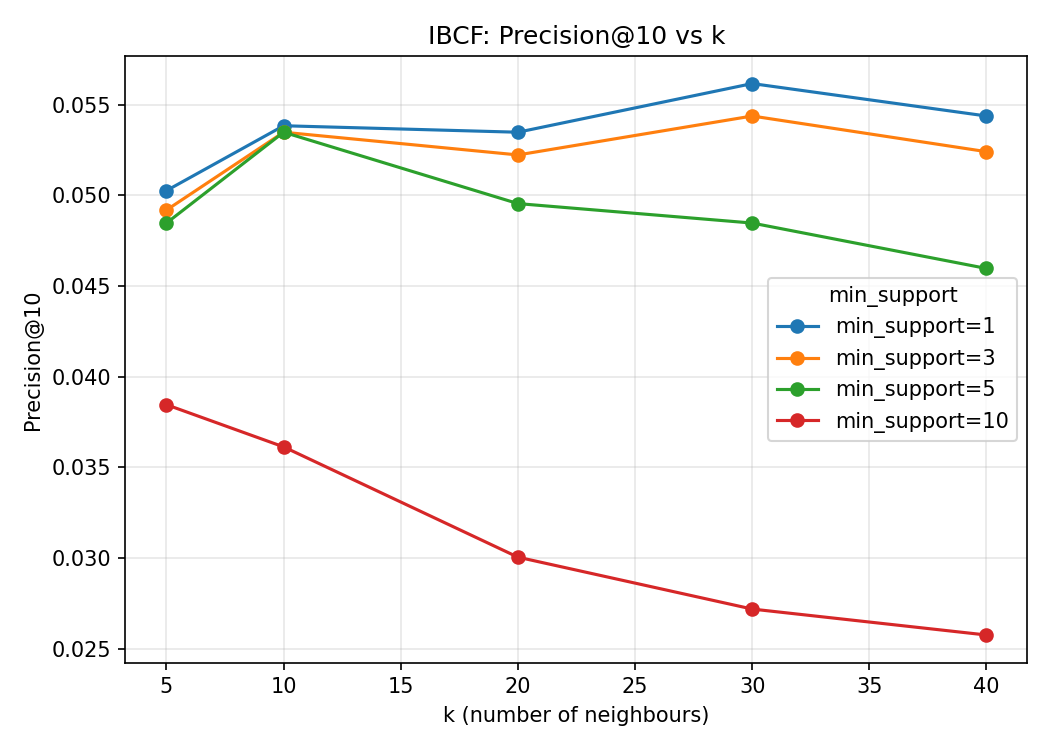
\includegraphics[width=\linewidth]{figures/ibcf_precision_vs_k.png}
\end{minipage}
\caption{RMSE and Precision@10 as a function of neighborhood size $k$, for each min\_support value tested. Top row: UBCF. Bottom row: IBCF.}
\label{fig:tuning}
\end{figure}

\subsection{Cold-Start and Sparsity Analysis}
To characterize behavior under limited data availability --- the classic ``cold-start'' scenario --- each user's training ratings were artificially truncated to a maximum of 1, 3, 5, 10, and 20 ratings, and RMSE was measured on the full test set for each truncation level (Table~\ref{tab:coldstart}).

\begin{table}[htbp]
\caption{RMSE Under Simulated Cold-Start Conditions}
\begin{center}
\begin{tabular}{|l|c|c|}
\hline
\textbf{Max ratings/user} & \textbf{UBCF RMSE} & \textbf{IBCF RMSE} \\
\hline
1 & 1.2605 & 1.2605 \\
\hline
3 & 1.0495 & 1.0571 \\
\hline
5 & 1.0031 & 1.0388 \\
\hline
10 & 0.9531 & 1.0705 \\
\hline
20 & 0.9337 & 1.0924 \\
\hline
Full (no truncation) & 0.8430 & 0.8769 \\
\hline
\end{tabular}
\label{tab:coldstart}
\end{center}
\end{table}

\begin{figure}[htbp]
\centerline{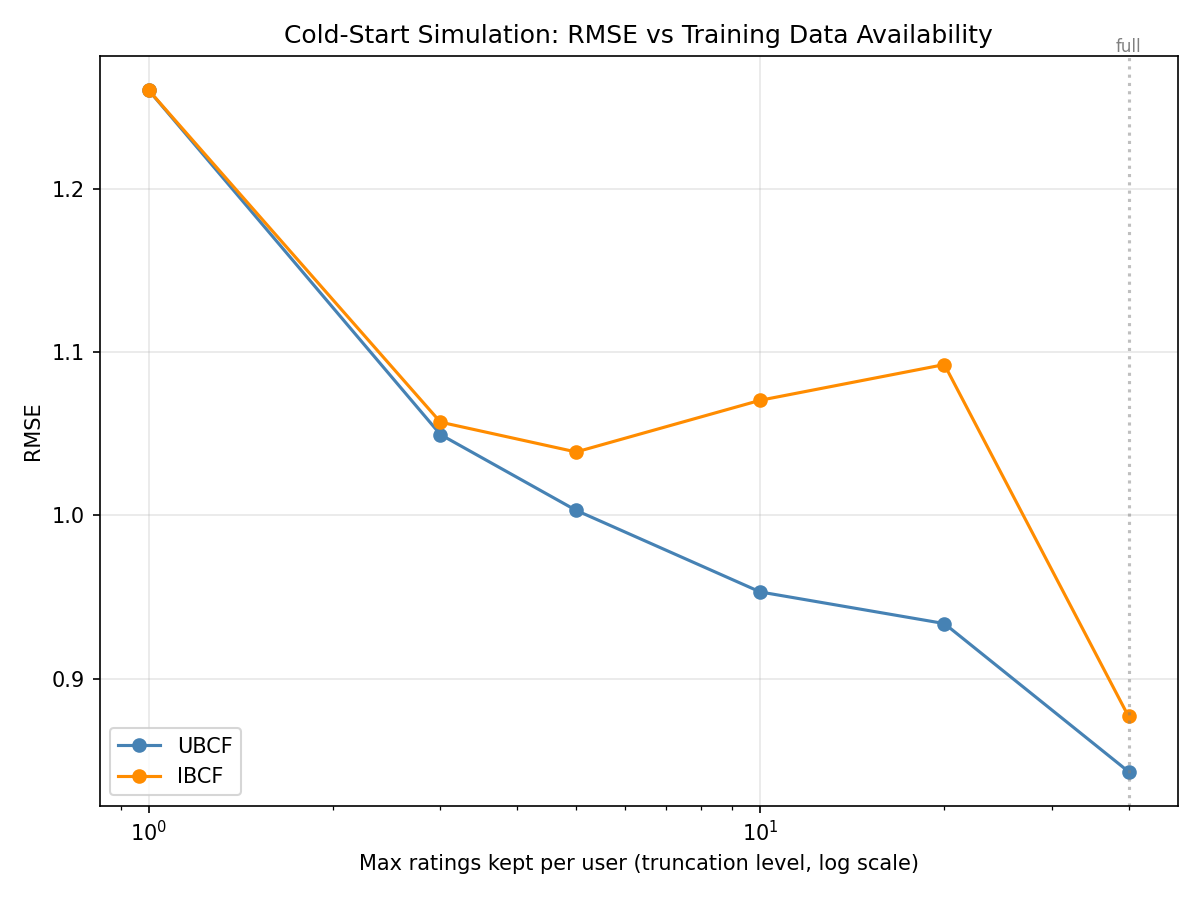
\includegraphics[width=\linewidth]{figures/cold_start_curve.png}}
\caption{RMSE vs. training data availability (simulated cold-start).}
\label{fig:coldstart}
\end{figure}

Fig.~\ref{fig:coldstart} plots this relationship. UBCF's RMSE decreases monotonically as more training data becomes available, matching the expected ``learning curve'' pattern. IBCF, however, displays non-monotonic behavior: RMSE improves through 5 ratings/user but then worsens at 10 and 20 before recovering sharply at full data. Investigation traced this to IBCF's tuned \texttt{min\_support} = 1 (Section~\ref{sec:tuning-results}): at very low data availability, almost no item pairs meet even this minimal co-rating threshold and predictions safely default to more stable estimates, but as truncation increases, progressively more item pairs clear the threshold on the strength of only one or two co-raters --- a statistically thin basis for similarity --- introducing noise that is only washed out once the full dataset restores adequate co-rating density. A controlled comparison using \texttt{min\_support} = 3 (IBCF's RMSE-optimal setting from Table~\ref{tab:tuning}) reduced the magnitude of the anomaly by more than half, though a smaller residual effect remained at the 10$\to$20 transition. This suggests \texttt{min\_support} is a substantial contributing factor, but not the only one.

A complementary analysis bucketed individual test predictions by the number of neighbors actually available at prediction time (Table~\ref{tab:neighbor}). For UBCF, RMSE decreases as neighbor support increases, consistent with the intuition that predictions backed by more corroborating evidence are more reliable.

\begin{table}[htbp]
\caption{UBCF Prediction RMSE Bucketed by Neighbor-Support Count\textsuperscript{a}}
\begin{center}
\begin{tabular}{|l|c|c|}
\hline
\textbf{Neighbor count bucket} & \textbf{UBCF RMSE} & \textbf{UBCF n} \\
\hline
0--2 & 1.1087 & 122 \\
\hline
3--5 & 0.9658 & 277 \\
\hline
6--10 & 0.9833 & 1{,}026 \\
\hline
11--20 & 0.8236 & 11{,}981 \\
\hline
\multicolumn{3}{l}{\footnotesize\textsuperscript{a}IBCF predictions were overwhelmingly concentrated in the} \\
\multicolumn{3}{l}{\footnotesize 11--20 and $>$20 buckets due to its low min\_support = 1,} \\
\multicolumn{3}{l}{\footnotesize precluding a comparable breakdown.}
\end{tabular}
\label{tab:neighbor}
\end{center}
\end{table}

\subsection{Scalability Analysis}
Model fit time was measured across four training-set sizes (25\%, 50\%, 75\%, 100\% of the training data); Fig.~\ref{fig:scalability} plots the result. Both models' fit time remained under 0.15 seconds even at full data size, with negligible growth across the range. This is because the number of distinct users and items is already saturated at 25\% of the data --- a direct consequence of the $\geq$20-ratings-per-entity filtering described in Section~\ref{sec:preprocessing} --- so the similarity matrices being computed do not grow further as more ratings are added. The substantial wall-clock difference observed during hyperparameter tuning (roughly 5--6 minutes per UBCF fit vs. 40--70 seconds per IBCF fit) was therefore not attributable to model fitting at all. Direct measurement of single-prediction latency revealed the true source: UBCF's \texttt{predict()} call takes approximately 0.593~ms on average, versus 0.064~ms for IBCF. This 9.2$\times$ difference comes from UBCF's prediction path relying on per-call pandas indexing operations, compared to IBCF's fully vectorized NumPy similarity lookups. This per-call overhead, multiplied across hundreds of candidate items per user during recommendation generation, reconstructs the empirically observed gap. Of the two neighborhood-based methods, IBCF therefore scales more favorably to larger user bases; the relative cost of UBCF comes from prediction-time implementation choices rather than an inherent limitation of the neighborhood-based approach itself.

\begin{figure}[htbp]
\centerline{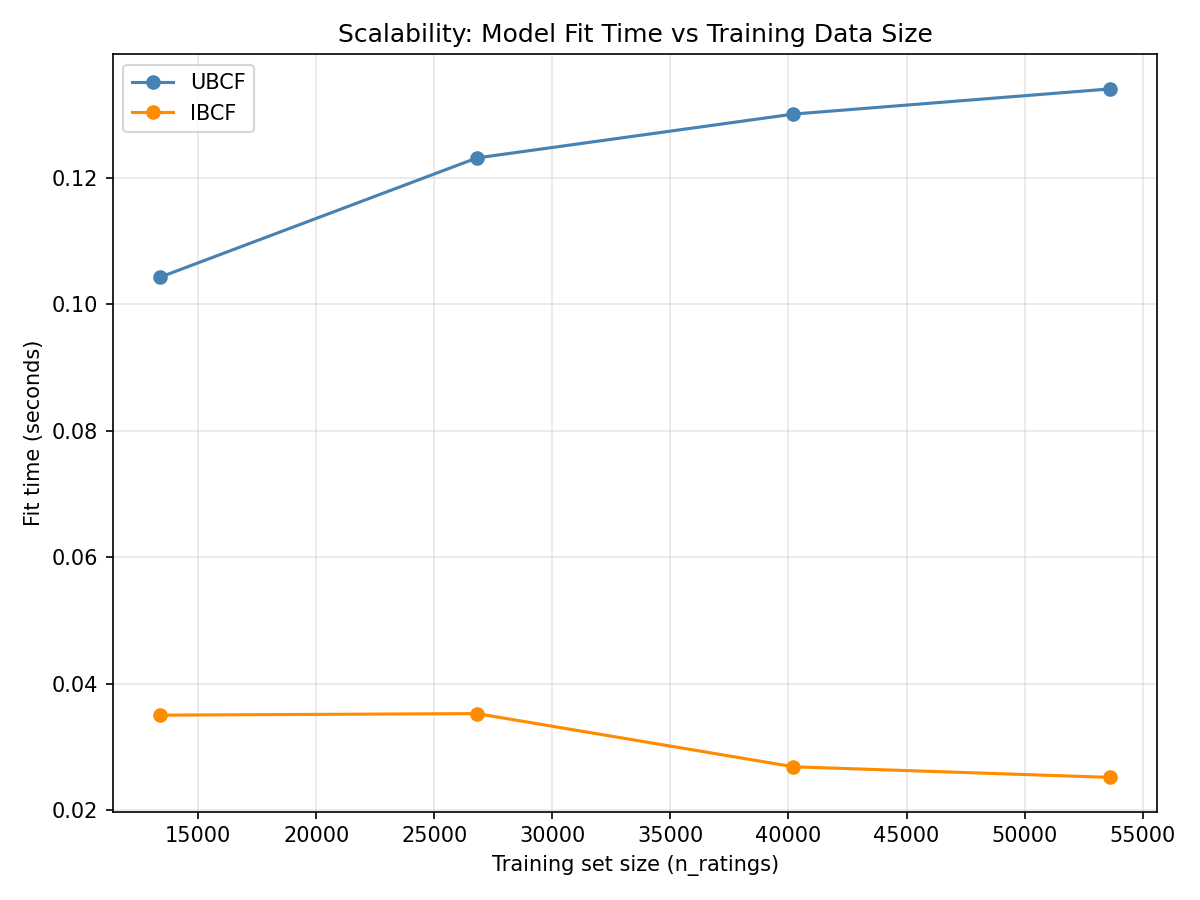
\includegraphics[width=\linewidth]{figures/scalability_curve.png}}
\caption{Model fit time as a function of training set size.}
\label{fig:scalability}
\end{figure}

\section{Discussion}

\subsection{Implementation Challenges}
\label{sec:impl}
Two implementation defects were found and fixed during development. Both were diagnosed systematically rather than by trial and error, and are documented here because they are the kind of mistake that is easy to make when implementing CF algorithms from first principles.

First, an early version of IBCF aggregated raw user ratings weighted by signed adjusted-cosine similarities ($\sum sim \cdot r / \sum |sim|$) rather than mean-centered deviations. Because adjusted cosine similarity can be negative, this formula allowed an item with strongly negative similarity but a high raw rating to contribute a large negative term to the numerator while still increasing the denominator, systematically pulling predictions toward the bottom of the rating scale; diagnostic analysis showed 45\% of a sample of test predictions clipping to the scale minimum (0.5) under this defect, with true ratings for those same items mostly in the 3--5 range. Replacing the formula with item-mean-centered deviations (Eq.~\eqref{eq:ibcf}, Section III-E) --- consistent with the standard formulation in Sarwar et al.~\cite{b2} --- resolved the issue, restoring RMSE from an initial 2.50 to the 0.87--0.88 range reported in Section IV-A.

Second, approximately 1.07\% of UBCF's raw (pre-clipping) predictions were found to exceed the upper bound of the rating scale, concentrated disproportionately among users with high personal mean ratings (a 4.1\% saturation rate for such users, versus the 1.07\% baseline). This was traced not to a coding error but to a mathematical property of the weighted-deviation formula (Eq.~\eqref{eq:ubcf}): because it is an additive combination of a mean and unbounded weighted deviations rather than a convex combination of ratings, it is not guaranteed to remain within [0.5, 5.0] when a user's neighbors show strong positive consensus. Clipping to the valid range, as implemented, is the correct and standard resolution. A secondary consequence was investigated: when multiple candidate recommendations clip to the same boundary value, their relative order in a top-K recommendation list becomes arbitrary unless explicitly broken. A deterministic tie-breaking rule --- ordering first by predicted score, then by the number of neighbors supporting that prediction, then by movie ID --- was added to ensure reproducible, non-arbitrary rankings among such ties.

\subsection{Limitations}
\label{sec:limitations}
\begin{itemize}
\item Both neighborhood models were tuned via grid search; SVD was evaluated with commonly-used default hyperparameters (50 factors, 20 epochs) without a comparable tuning phase. SVD's already-superior performance may understate its true advantage relative to a tuned configuration, a question left open for future work.
\item The dataset's aggressive filtering ($\geq$20 ratings per user and per movie, Section III-B) deliberately excludes the most extreme cold-start cases from the primary evaluation; the cold-start analysis in Section IV-D uses artificial truncation of otherwise-eligible users' histories as a proxy, which may not perfectly represent the behavior of an actual new user or item in a live system.
\item Precision@K and Recall@K were computed using a fixed relevance threshold (rating $\geq$ 4.0); results may differ under alternative thresholds, and this was not explored as a sensitivity analysis.
\item The residual (partially unexplained) component of IBCF's cold-start non-monotonicity (Section IV-D) was investigated but not fully resolved; a smaller effect persisted even after controlling for \texttt{min\_support}, suggesting an additional contributing mechanism not yet identified.
\item Evaluation was conducted on a single fixed train/test split (with a bootstrap resampling test applied post hoc for significance); k-fold cross-validation was not performed and would provide a more complete picture of variance across different data partitions.
\end{itemize}

\section{Conclusion and Future Work}
This project implemented and evaluated two collaborative filtering approaches, User-Based and Item-Based CF, from first principles, alongside three non-personalized baselines and an SVD comparison. Both personalized neighborhood models clearly outperformed the non-personalized baselines, and the bootstrap test showed that UBCF's RMSE advantage over IBCF, although numerically small ($\approx$0.034), is statistically significant rather than a split-dependent fluke. SVD had the best overall numbers, in line with prior work on matrix factorization, but it was not tuned to the same extent as UBCF and IBCF, so this comparison is not entirely fair to the neighborhood-based models. The cold-start and neighbor-support experiments confirmed that neighborhood methods are sensitive to data sparsity: UBCF degraded predictably as data was removed, while IBCF's behavior was more complex and only partially explained by its tuned \texttt{min\_support} value. The scalability analysis showed that the practical speed difference between UBCF and IBCF comes from prediction-time implementation choices (pandas vs. NumPy), not from an inherent limitation of the neighborhood-based approach.

Future work could extend this study in several directions: running a comparable hyperparameter search for the SVD model, using k-fold cross-validation to assess variance across data partitions, running a sensitivity analysis on the relevance threshold used for the ranking metrics, and further isolating the unexplained part of IBCF's cold-start behavior noted in Section~\ref{sec:limitations}. The implementation --- including 104 automated unit and integration tests, a reproducible pipeline, and an interactive demonstration interface --- is available in the project's version-controlled repository.

\begin{thebibliography}{00}
\bibitem{b1} P. Resnick, N. Iacovou, M. Suchak, P. Bergstrom, and J. Riedl, ``GroupLens: An Open Architecture for Collaborative Filtering of Netnews,'' in \textit{Proc. ACM Conf. Computer Supported Cooperative Work (CSCW)}, 1994, pp. 175--186.
\bibitem{b2} B. Sarwar, G. Karypis, J. Konstan, and J. Riedl, ``Item-Based Collaborative Filtering Recommendation Algorithms,'' in \textit{Proc. 10th Int. Conf. World Wide Web (WWW)}, 2001, pp. 285--295.
\bibitem{b3} F. M. Harper and J. A. Konstan, ``The MovieLens Datasets: History and Context,'' \textit{ACM Trans. Interactive Intelligent Systems}, vol. 5, no. 4, article 19, Dec. 2015.
\bibitem{b4} N. Hug, ``Surprise: A Python Library for Recommender Systems,'' \textit{Journal of Open Source Software}, vol. 5, no. 52, p. 2174, 2020.
\bibitem{b5} Y. Koren, R. Bell, and C. Volinsky, ``Matrix Factorization Techniques for Recommender Systems,'' \textit{IEEE Computer}, vol. 42, no. 8, pp. 30--37, Aug. 2009.
\end{thebibliography}

\end{document}
